\documentclass[a4paper]{article}
\usepackage{ctex}
\usepackage[affil-it]{authblk}
\usepackage[backend=bibtex,style=numeric]{biblatex}
\usepackage{amsmath,amsthm,amssymb,amsfonts}
\usepackage{graphicx}
\usepackage{bm}
\usepackage{float}
\usepackage{geometry}
\geometry{margin=1.5cm, vmargin={0pt,1cm}}
\setlength{\topmargin}{-1cm}
\setlength{\paperheight}{29.7cm}
\setlength{\textheight}{25.3cm}

\addbibresource{citation.bib}

\begin{document}
% =================================================
\title{微分方程数值解 2026 春夏编程作业一}

\author{曾申昊 3220100701
  \thanks{邮箱: \texttt{3097714673@qq.com}
                            \texttt{或} \texttt{3220100701@zju.edu.cn}}}
\affil{浙江大学}

\date{更新时间: \today}

\maketitle

% ============================================

\section{理论分析}

\par 对于内部点采用五点差分格式，对于边界点则需要根据边界条件来推导差分格式。
矩形Dirichlet边界处的差分格式比较简单，直接用该点处的精确值来消去即可，
对于剩下三种边界条件的差分格式推导如下：

\subsection{矩形Neumann边界处的差分格式}
\par 将矩形Neumann边界条件具体分量写出： 
\begin{equation}
    \left\{
        \begin{aligned}
            &-\frac{\partial u}{\partial x}\bigg|_{x=0} = g_1(y)\\
            &\frac{\partial u}{\partial x}\bigg|_{x=1} = g_2(y)\\
            &-\frac{\partial u}{\partial y}\bigg|_{y=0} = g_3(x)\\
            &\frac{\partial u}{\partial y}\bigg|_{y=1} = g_4(x)\\
        \end{aligned}
    \right.
\end{equation}
\par 以$-\dfrac{\partial u}{\partial x}\bigg|_{x=0} = g_1(y)$为例有
\begin{equation}
    \left\{
        \begin{gathered}
            \frac{1}{h^2}\left[
                4U(0, j) - U(0, j+1) - U(0, j-1) - U(1, j) - U(-1, j)
            \right]=f(0,jh)\\
            \frac{-1}{2h}\left[
                U(1, j) - U(-1, j)
            \right] = g_1(jh)
        \end{gathered}
    \right.
\end{equation}
\par 消去 $U(-1, j)$ 后得到
\begin{equation}
    \begin{gathered}
        \frac{1}{h^2}\left[
            4U(0, j) - U(0, j+1) - U(0, j-1) - 2U(1, j) - 2hg_1(jh)
        \right]=f(0,jh)\\
        \frac{1}{h^2}\left[
            4U(0, j) - U(0, j+1) - U(0, j-1) - 2U(1, j)
        \right]=f(0,jh)+\frac{2}{h}g_1(jh)
    \end{gathered}
\end{equation}
\par 其他边界处的差分格式同理可得，如果五点差分格式中有
矩形角点：
\begin{equation}
    \frac{1}{h^2}\left[
        4U(0, 1) - U(0, 2) - U(0, 0) - 2U(1, 1)
    \right]=f(0,h)+\frac{2}{h}g_1(h)
\end{equation}
\par 因为一般情况下的五点差分格式是用不到矩形角点的，
所以在具体编程时是直接用 $u(0,0)$ 精确值来消去的。

\subsection{圆形Dirichlet边界处的差分格式}

\begin{figure}
    \centering
    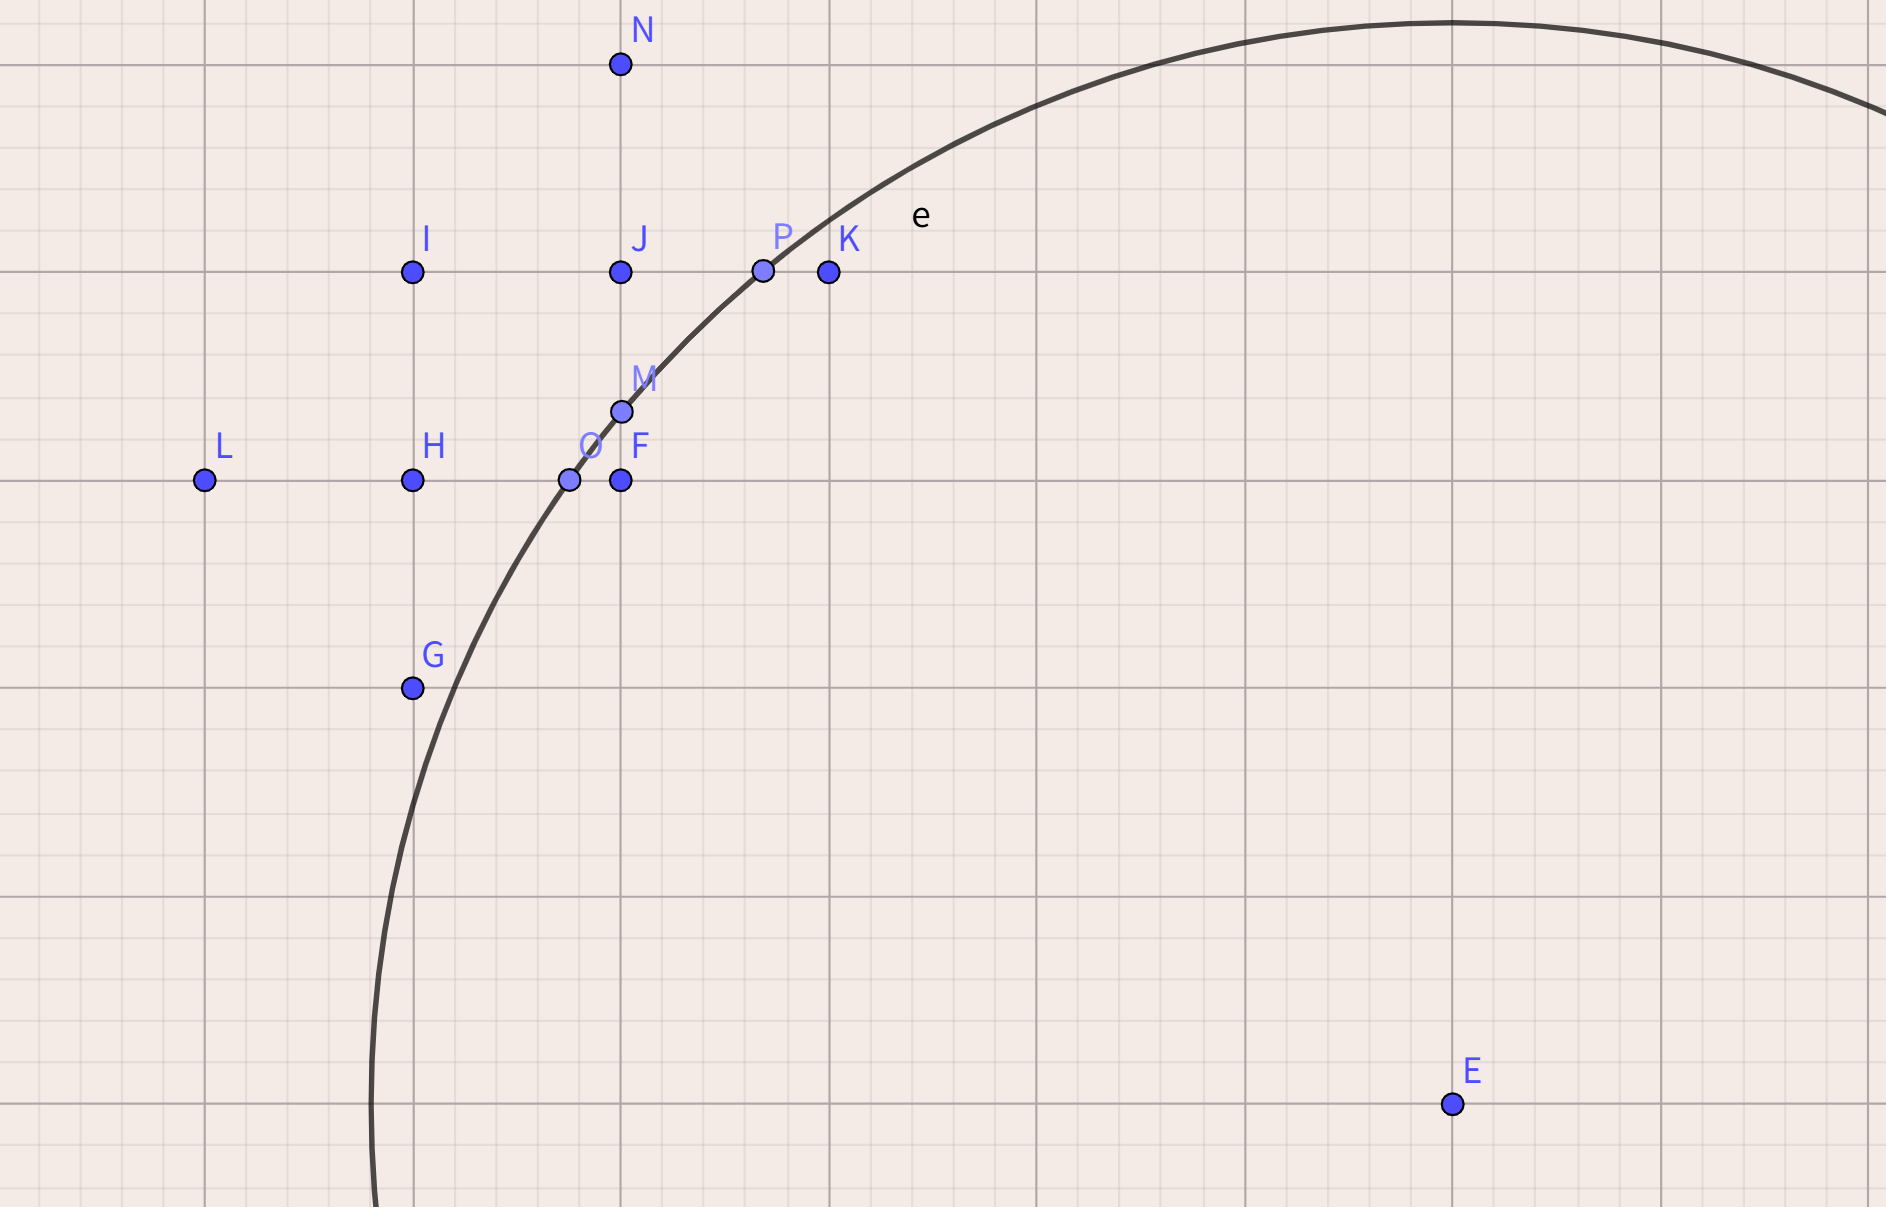
\includegraphics[width=0.7\textwidth]{figure/Circle_Dirichlet.png}
    \caption{圆形Dirichlet边界处的差分格式示意图}
    \label{fig:Circle_Dirichlet}
\end{figure}

\par 如图\ref{fig:Circle_Dirichlet}所示，以$J$点为例，
它的五点差分格式中包括$K$点和$F$点，而这两点位于圆内，需要利用 Dirichlet 边界条件来消去。
线段$JK$与圆相交于$P$点，线段$JF$与圆相交于$M$点。
记 $|JP|=\alpha h$，$|JM|=\theta h$，
根据讲义上不规则边界的差分格式有：
\begin{equation}
    \frac{(1+\alpha)U_J-U_P-\alpha U_I}{\frac{1}{2}\alpha(1+\alpha)h^2}
    +\frac{(1+\theta)U_J-U_M-\theta U_N}{\frac{1}{2}\theta(1+\theta)h^2}
    =f(x_J,y_J)
\end{equation}
\par 用圆形边界处的精确值来消去 $U_P$ 和 $U_M$ 后得到
\begin{equation}    
    \frac{(1+\alpha)U_J-\alpha U_H}{\frac{1}{2}\alpha(1+\alpha)h^2}
    +\frac{(1+\theta)U_J-\theta U_K}{\frac{1}{2}\theta(1+\theta)h^2}
    =f(x_J,y_J)+\frac{2}{h^2}\left(
        \frac{u(x_P,y_P)}{\alpha(1+\alpha)} + \frac{u(x_M,y_M)}{\theta(1+\theta)}
    \right)
\end{equation}
\par 对于图中的 $H$ 点，它的五点差分格式中只有 $F$ 点在圆内，
线段$HF$与圆相交于$O$点，记$|HO|=\beta h$，
相应的差分格式同样可以写成上面的形式：
\begin{equation}
    \begin{gathered}
        \frac{(1+\beta)U_H-U_O-\beta U_L}{\frac{1}{2}\beta(1+\beta)h^2}
        +\frac{2U_H-U_I-U_G}{h^2}
        =f(x_H,y_H)\\
        \frac{(1+\beta)U_H-\beta U_L}{\frac{1}{2}\beta(1+\beta)h^2}
        +\frac{2U_H-U_I-U_G}{h^2}
        =f(x_H,y_H)+\frac{2}{h^2}
        \frac{u(x_O,y_O)}{\beta(1+\beta)}
    \end{gathered}
\end{equation}

\subsection{圆形Neumann边界处的差分格式}
\begin{figure}
    \centering
    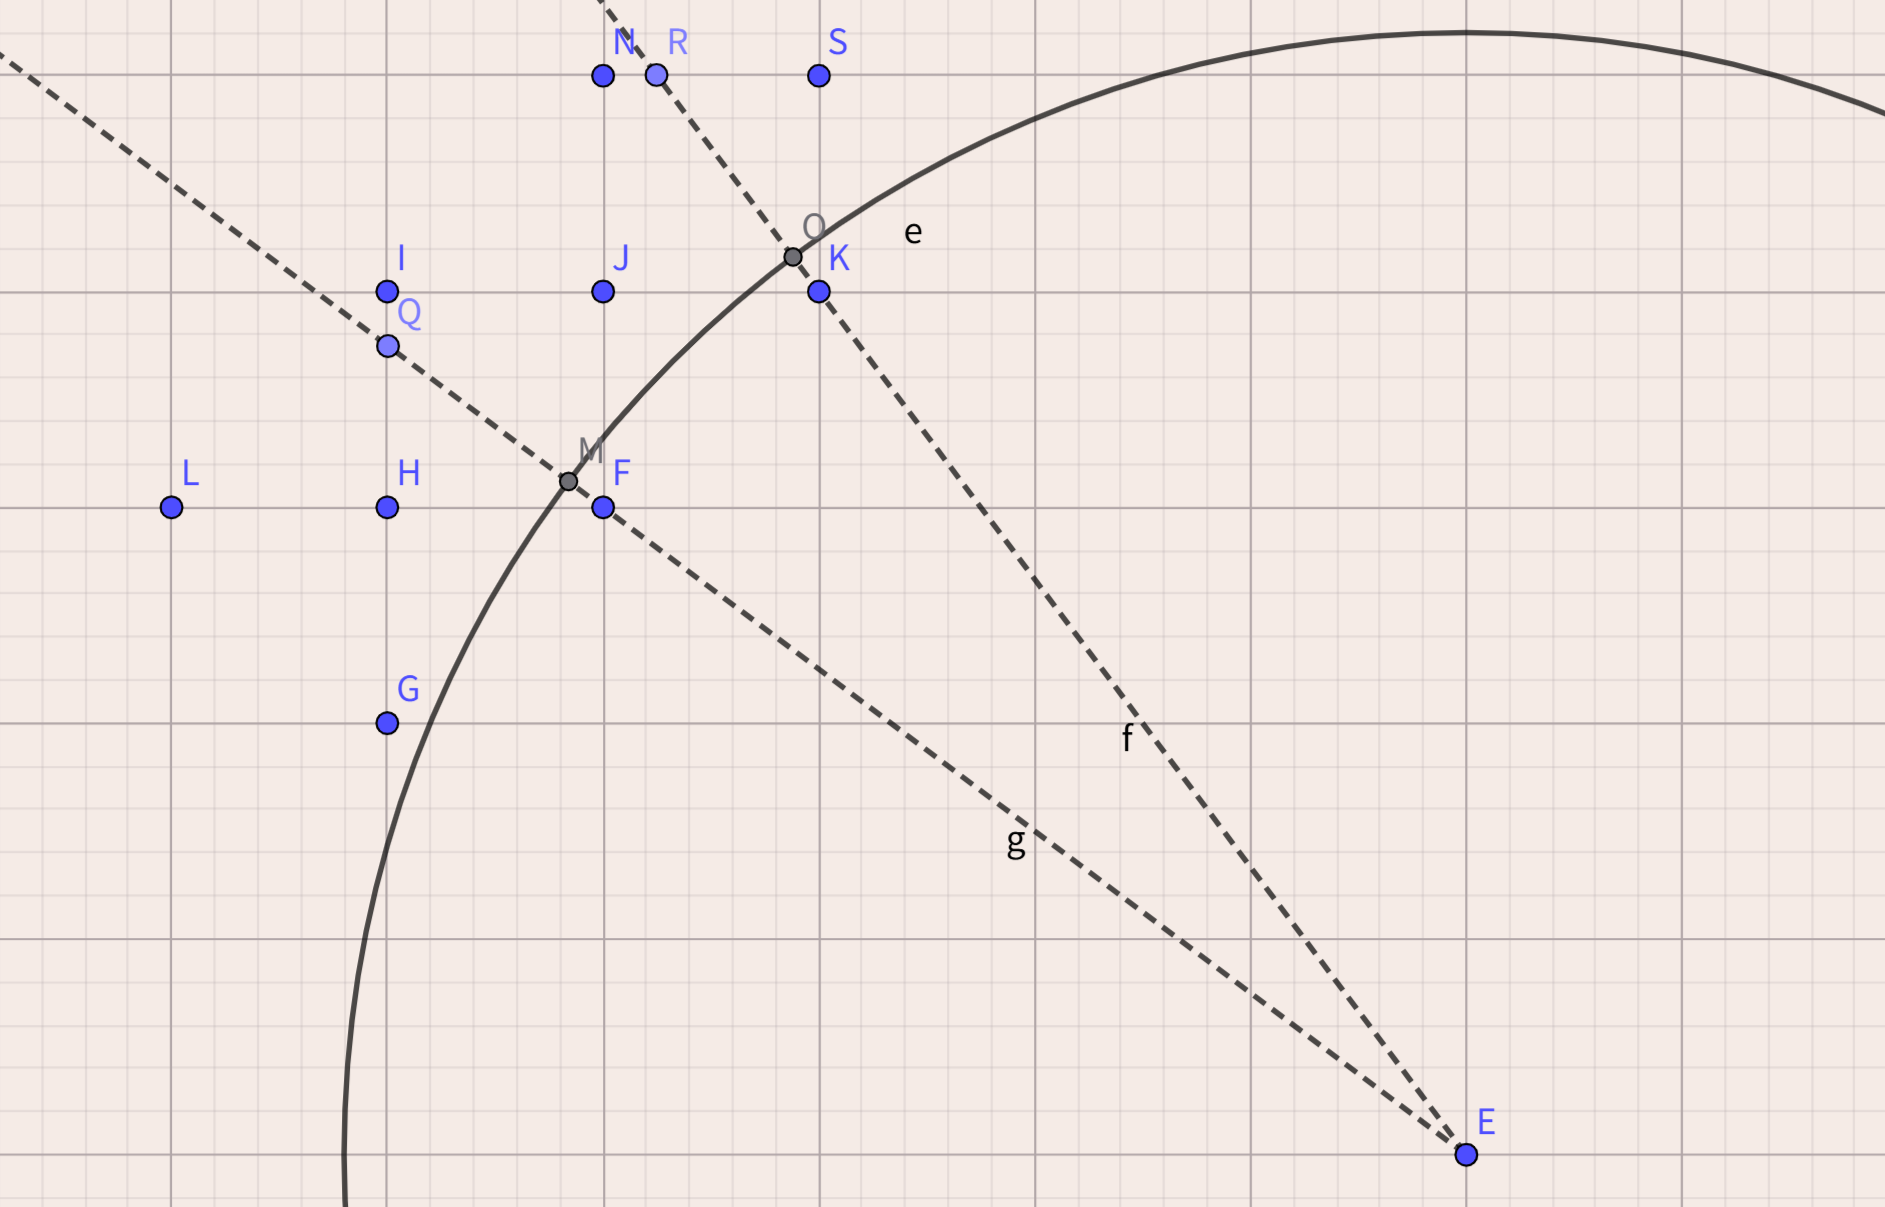
\includegraphics[width=0.7\textwidth]{figure/Circle_Neumman.png}
    \caption{圆形Neumann边界处的差分格式示意图}
    \label{fig:Circle_Neumman}
\end{figure}
\par 如图\ref{fig:Circle_Neumman}所示，以$H$点为例，
它的五点差分格式中包括$F$点，而$F$点在圆内，需要利用 Neumann 边界条件来消去。
作圆心到$F$点的延长线，与圆相交于$M$点，并与 $H$ 点的垂直线相交于$Q$点，
记 $\left|FQ\right|=d$。
利用 $U_F$ 点和 $U_Q$ 点的值来计算 Neumann 边界条件的数值近似值，
并用 $U_I$ 和 $U_H$ 的线性插值来近似 $U_Q$：
\begin{equation}
    \left\{
        \begin{gathered}
            \frac{1}{h^2}\left[
                4U_H - U_L - U_F - U_I - U_G
            \right]=f(x_H,y_H)\\
            \frac{1}{d}\left[
                U_F - U_Q
            \right] = g(x_M,y_M)\\
            U_{G'} = w_1 U_H + w_2 U_I
        \end{gathered}
    \right.
\end{equation}
\par 消去 $U_G$ 和 $U_{G'}$ 后得到
\begin{equation}
    \begin{gathered}
        \frac{1}{h^2}\left[
            4U_H - U_L - U_I - U_G - (U_Q + dg(x_M,y_M))
        \right]=f(x_H,y_H)\\
        \frac{1}{h^2}\left[
            4U_H - U_L - U_I - U_G - \left(
                w_1 U_H + w_2 U_I
            \right)
        \right]=f(x_H,y_H)
        +\frac{d}{h^2}g(x_M,y_M)
    \end{gathered}
\end{equation}
\par 对于 $J$ 点来说，
它的五点差分格式中有两点位于圆内，消去后得到的差分格式同样可以写成上面的形式。
\begin{equation}
    \frac{1}{h^2}\left[
        4U_J - U_I - U_N - \left(
            w_1 U_H + w_2 U_I
        \right)
        -\left(
            w_3 U_N + w_4 U_S
        \right)
    \right]=f(x_J,y_J)
    +\frac{d}{h^2}g(x_M,y_M)
    +\frac{d}{h^2}g(x_O,y_O)
\end{equation}

\section{数值结果}

\subsection{第一个测试函数}

\par 第一个测试函数为：
\begin{equation}
    u(x,y)=e^{y+\sin x}
\end{equation}
\par 对于第一种边界假设：纯 Dirichlet 条件、计算域为一个完整的矩形。
\begin{table}[H]
    \centering
    \begin{tabular}{|c|c|c|c|}    
    \hline
    n& 1-norm & 2-norm & $\infty$-norm  \\ \hline
    8&  1.81462e-04&  2.27076e-04 & 4.39017e-04  \\ \hline
    16& 5.19977e-05 & 6.35612e-05 & 1.19262e-04 \\ \hline
    32& 1.30391e-05 & 1.56467e-05 & 3.10786e-05 \\ \hline
    64& 3.72382e-06 & 4.5851e-06 &  8.94185e-06 \\ \hline
    \end{tabular}
\end{table}
\begin{figure}[H]
    \centering
    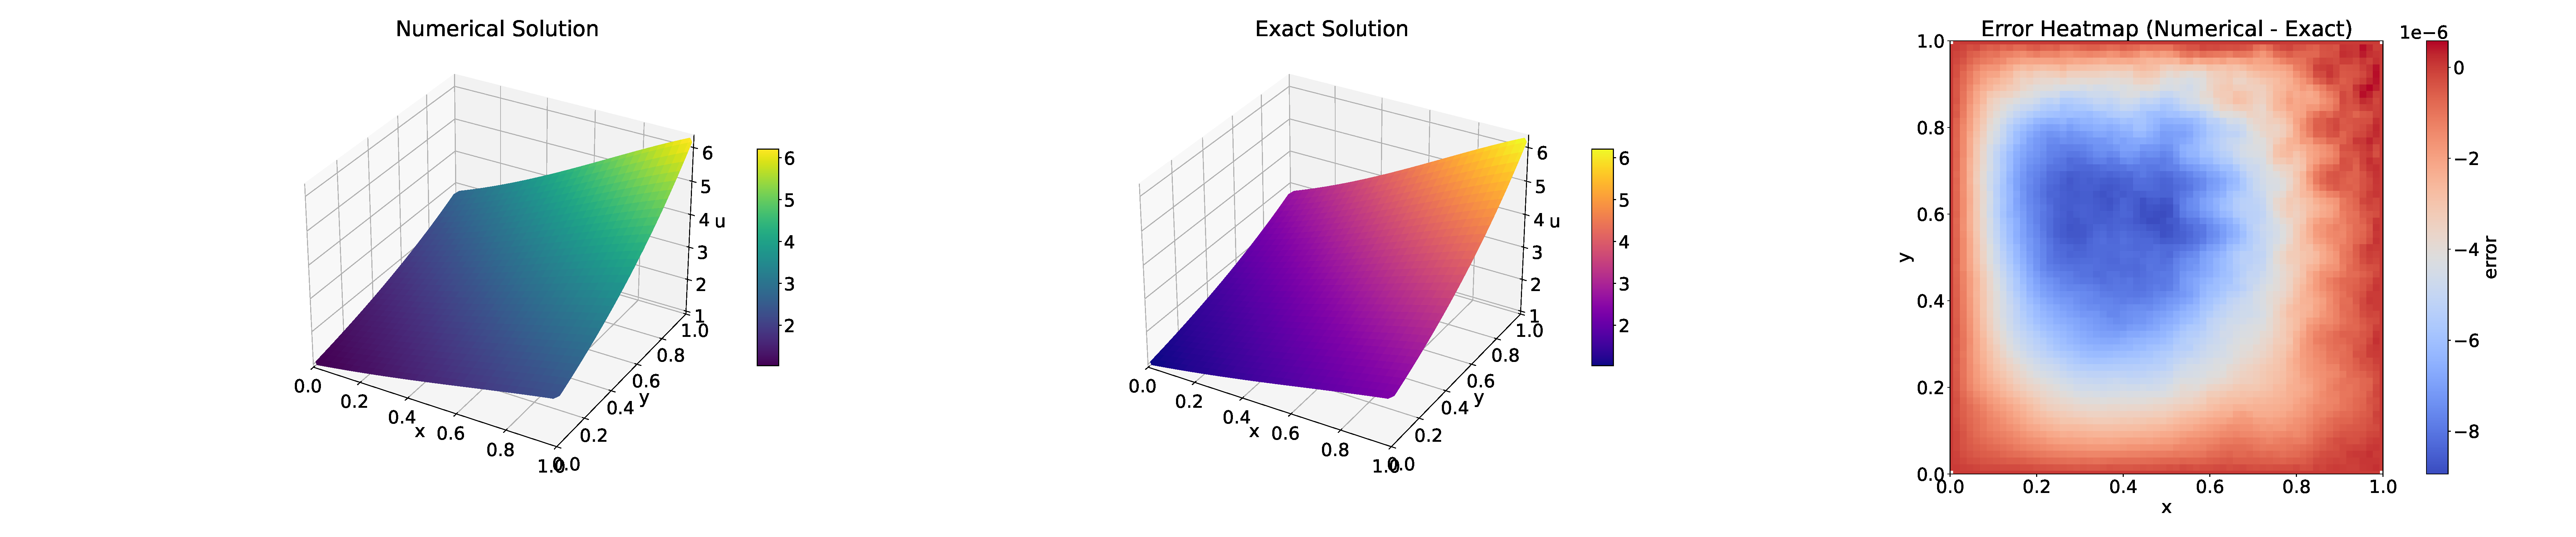
\includegraphics[width=1\textwidth]{figure/PureDirchlet_Rectangle_Function1.pdf}
    \caption{第一个测试函数：第一种边界假设}
    \label{fig:PureDirchlet_Rectangle_Function1}
\end{figure}
\par 对于第二种边界假设：纯 Dirichlet 条件、计算域为一个矩形挖去一个圆形
$(x-0.5)^2+(y-0.5)^2=0.04$
\begin{table}[H]
    \centering
    \begin{tabular}{|c|c|c|c|}    
    \hline
    n& 1-norm & 2-norm & $\infty$-norm  \\ \hline
    8&  5.49155e-05&  8.44303e-05 & 2.70863e-04  \\ \hline
    16& 1.35892e-05 & 1.74182e-05 & 5.21146e-05 \\ \hline
    32& 3.17729e-06 & 3.97888e-06 & 1.05642e-05 \\ \hline
    64& 9.62661e-07 & 1.3499e-06 &  4.27728e-06 \\ \hline
    \end{tabular}
\end{table}
\begin{figure}[H]
    \centering
    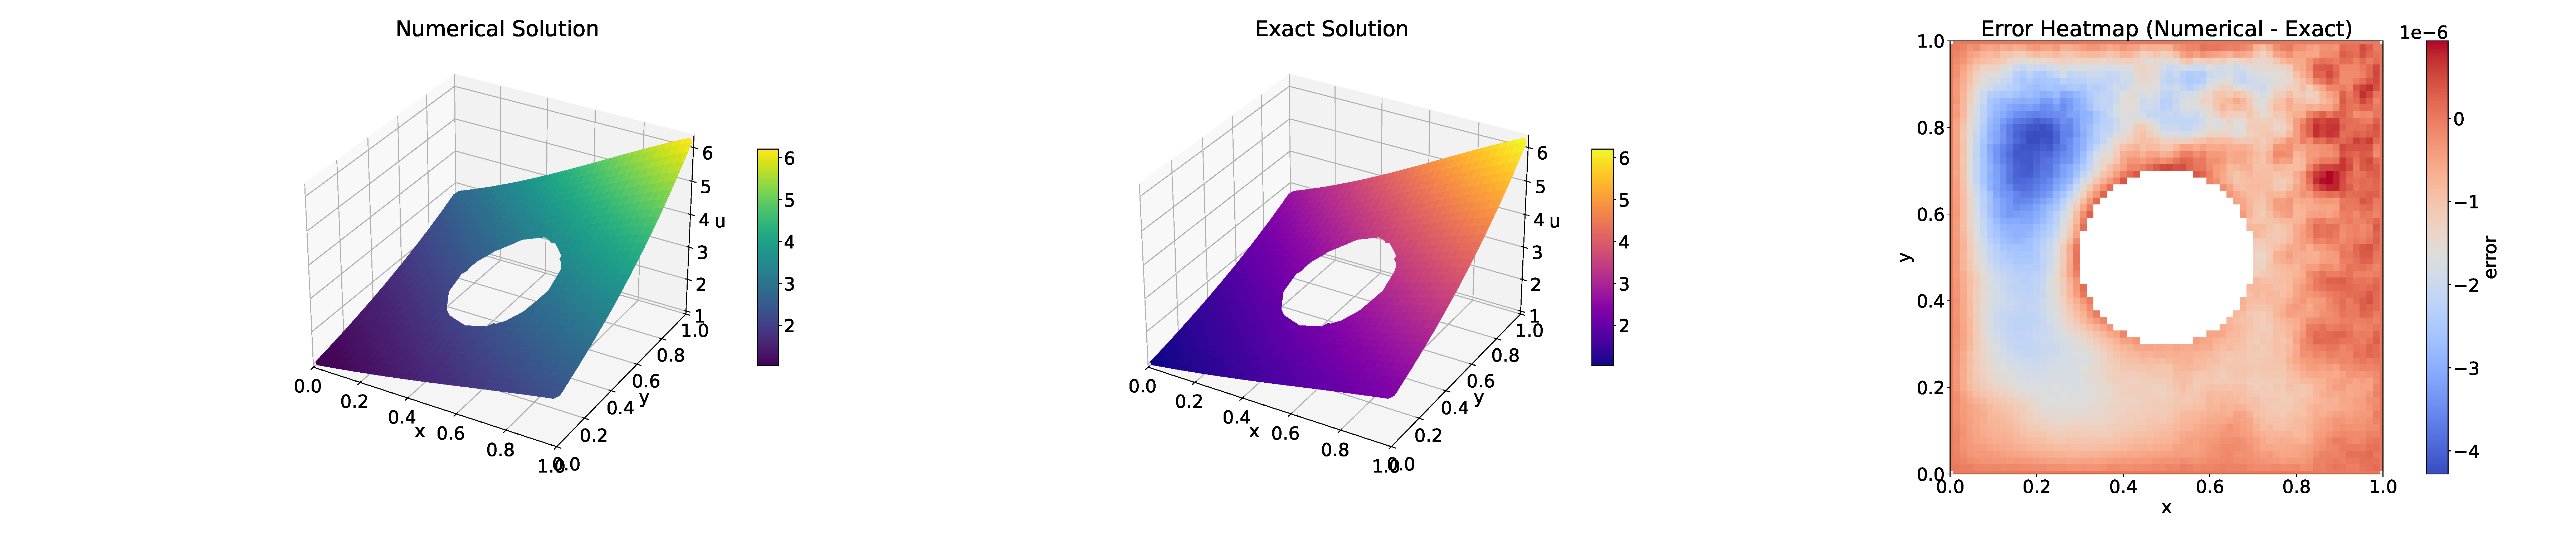
\includegraphics[width=1\textwidth]{figure/PureDirchlet_Circle_Function1.pdf}
    \caption{第一个测试函数：第二种边界假设}
    \label{fig:PureDirchlet_Circle_Function1}
\end{figure}
\par 对于第三种边界假设：矩形左右两边为 Neumann条件，
其余为 Dirichlet 条件、计算域为一个矩形挖去一个圆形
$(x-0.5)^2+(y-0.5)^2=0.04$
\begin{table}[H]
    \centering
    \begin{tabular}{|c|c|c|c|}    
    \hline
    n& 1-norm & 2-norm & $\infty$-norm  \\ \hline
    8&  6.42517e-04&  1.23533e-03 & 4.09898e-03  \\ \hline
    16& 1.70297e-04 & 3.25303e-04 & 1.18141e-04 \\ \hline
    32& 4.14486e-05 & 7.98462e-05 & 3.10637e-04 \\ \hline
    64& 1.15238e-05 & 2.14003e-05 &  8.57097e-05 \\ \hline
    \end{tabular}
\end{table}
\begin{figure}[H]
    \centering
    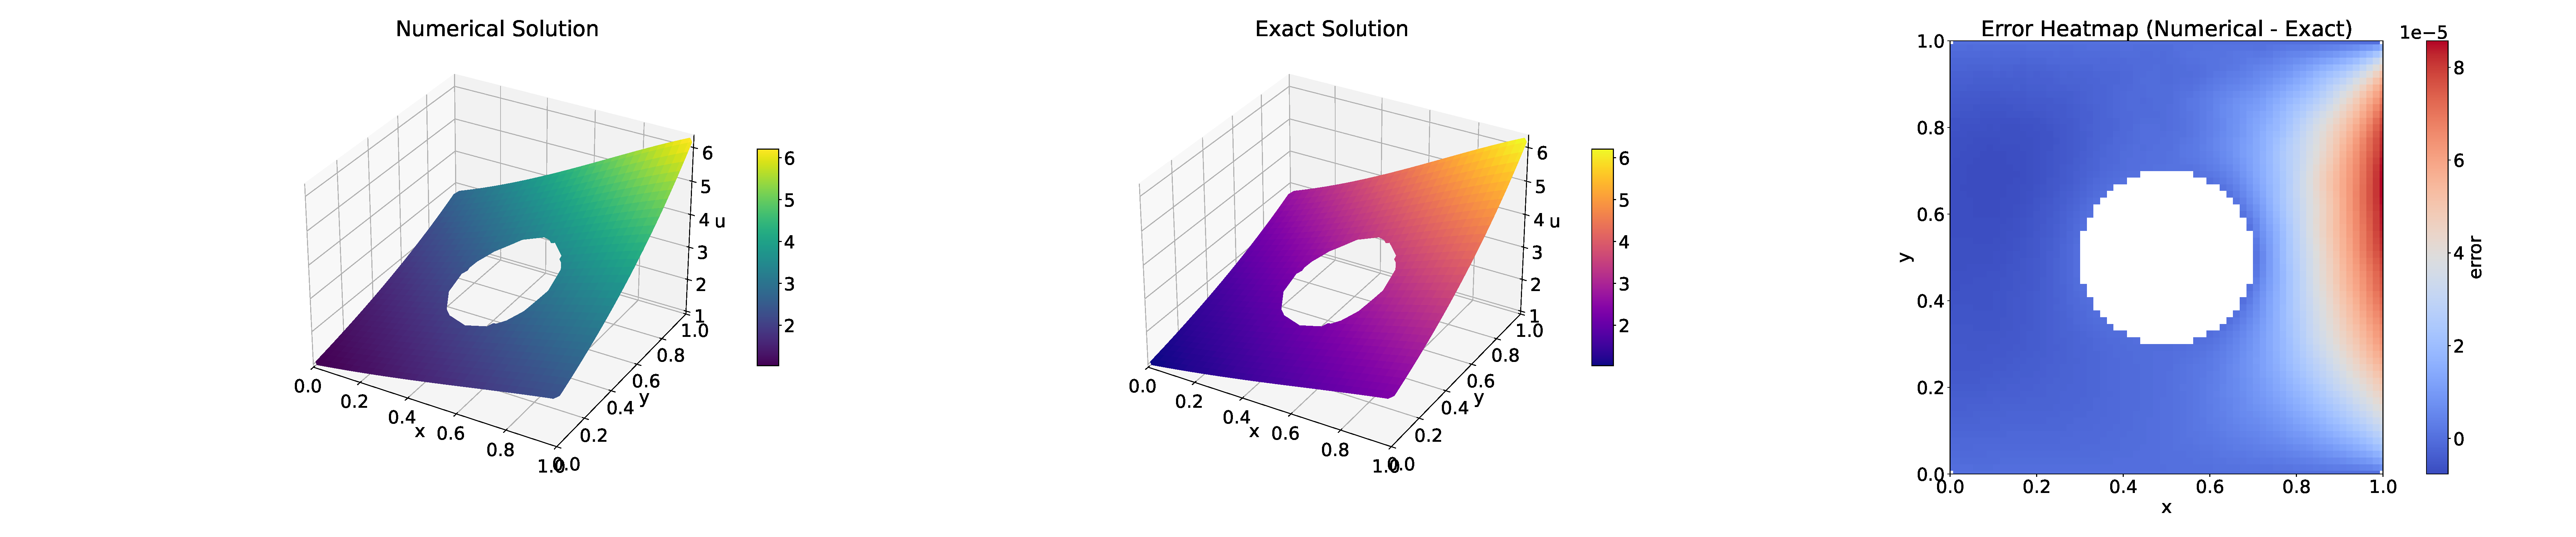
\includegraphics[width=1\textwidth]{figure/MixedNeumann_Rectangle_Function1.pdf}
    \caption{第一个测试函数：第三种边界假设}
    \label{fig:MixedNeumann_Rectangle_Function1}
\end{figure}
\par 对于第四种边界假设：圆形为 Neumann条件，
其余为 Dirichlet 条件、计算域为一个矩形挖去一个圆形
$(x-0.5)^2+(y-0.5)^2=0.04$
\begin{table}[H]
    \centering
    \begin{tabular}{|c|c|c|c|}    
    \hline
    n& 1-norm & 2-norm & $\infty$-norm  \\ \hline
    8&  0.00411967&  0.00623504 & 0.0207507  \\ \hline
    16& 0.000329704 & 0.000612089 & 0.00321633 \\ \hline
    32& 0.00111555 & 0.00168861 & 0.00803162 \\ \hline
    64& 0.000534312 & 0.000802221 &  0.00382181 \\ \hline
    \end{tabular}
\end{table}
\begin{figure}[H]
    \centering
    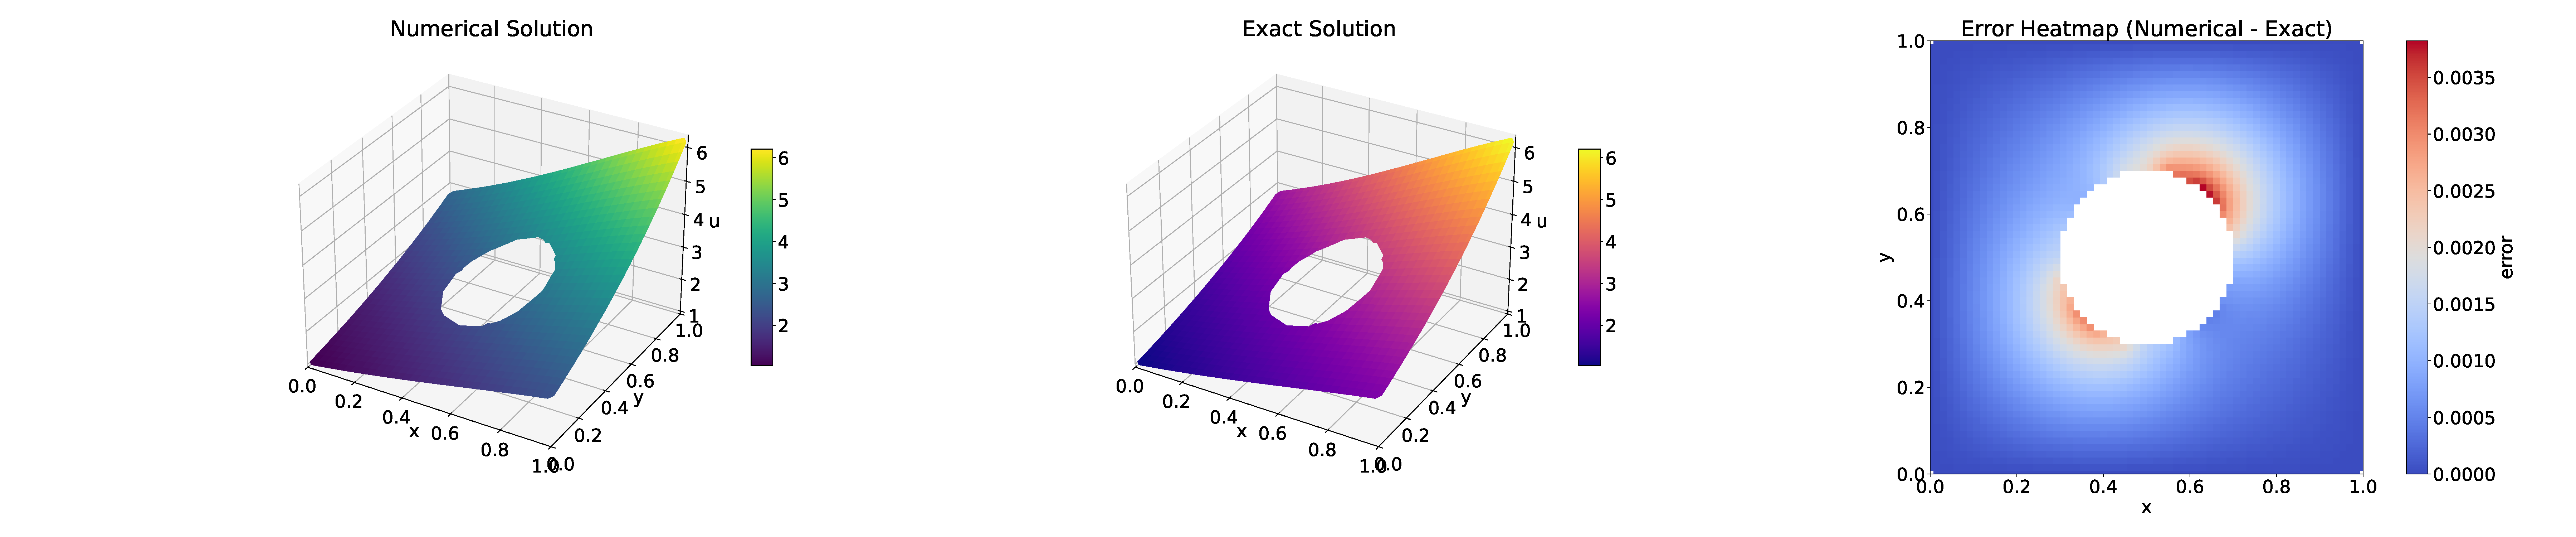
\includegraphics[width=1\textwidth]{figure/MixedNeumann_Circle_Function1.pdf}
    \caption{第一个测试函数：第四种边界假设}
    \label{fig:MixedNeumann_Circle_Function1}
\end{figure}

\subsection{第二个测试函数}

\par 第二个测试函数为：
\begin{equation}
    u(x,y)=x(1-x)y(1-y)
\end{equation}
\par 对于第一种边界假设：纯 Dirichlet 条件、计算域为一个完整的矩形。
\begin{table}[H]
    \centering
    \begin{tabular}{|c|c|c|c|}    
    \hline
    n& 1-norm & 2-norm & $\infty$-norm  \\ \hline
    8&  4.96415e-08&  7.61458e-08 & 2.11184e-07  \\ \hline
    16& 3.92053e-08 & 5.15786e-08 & 1.51537e-07 \\ \hline
    32& 4.86972e-08 & 6.41683e-08 & 1.52673e-07 \\ \hline
    64& 8.71658e-09 & 1.14751e-08 &  3.40448e-08 \\ \hline
    \end{tabular}
\end{table}
\begin{figure}[H]
    \centering
    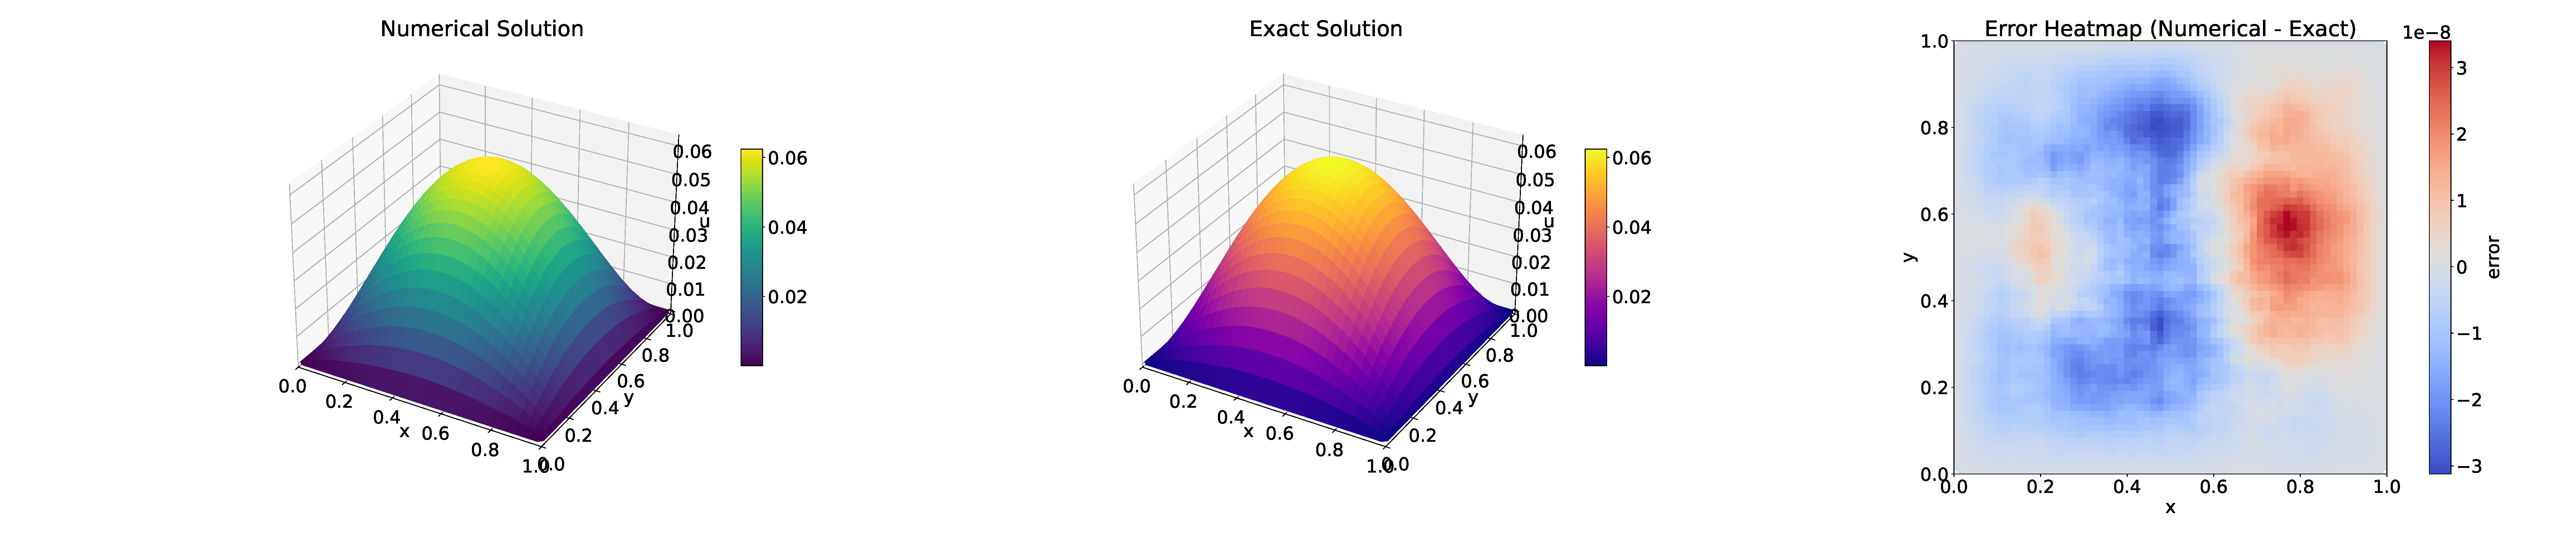
\includegraphics[width=1\textwidth]{figure/PureDirchlet_Rectangle_Function2.pdf}
    \caption{第二个测试函数：第一种边界假设}
    \label{fig:PureDirchlet_Rectangle_Function2}
\end{figure}
\par 对于第二种边界假设：纯 Dirichlet 条件、计算域为一个矩形挖去一个圆形
$(x-0.5)^2+(y-0.5)^2=0.04$
\begin{table}[H]
    \centering
    \begin{tabular}{|c|c|c|c|}    
    \hline
    n& 1-norm & 2-norm & $\infty$-norm  \\ \hline
    8&  2.35932e-08&  3.93263e-08 & 1.34549e-07  \\ \hline
    16& 2.29068e-08 & 3.27553e-08 & 8.48465e-08 \\ \hline
    32& 5.58752e-09 & 8.60063e-09 & 3.9366e-08 \\ \hline
    64& 4.67003e-09 & 6.85491e-09 &  2.56805e-08 \\ \hline
    \end{tabular}
\end{table}
\begin{figure}[H]
    \centering
    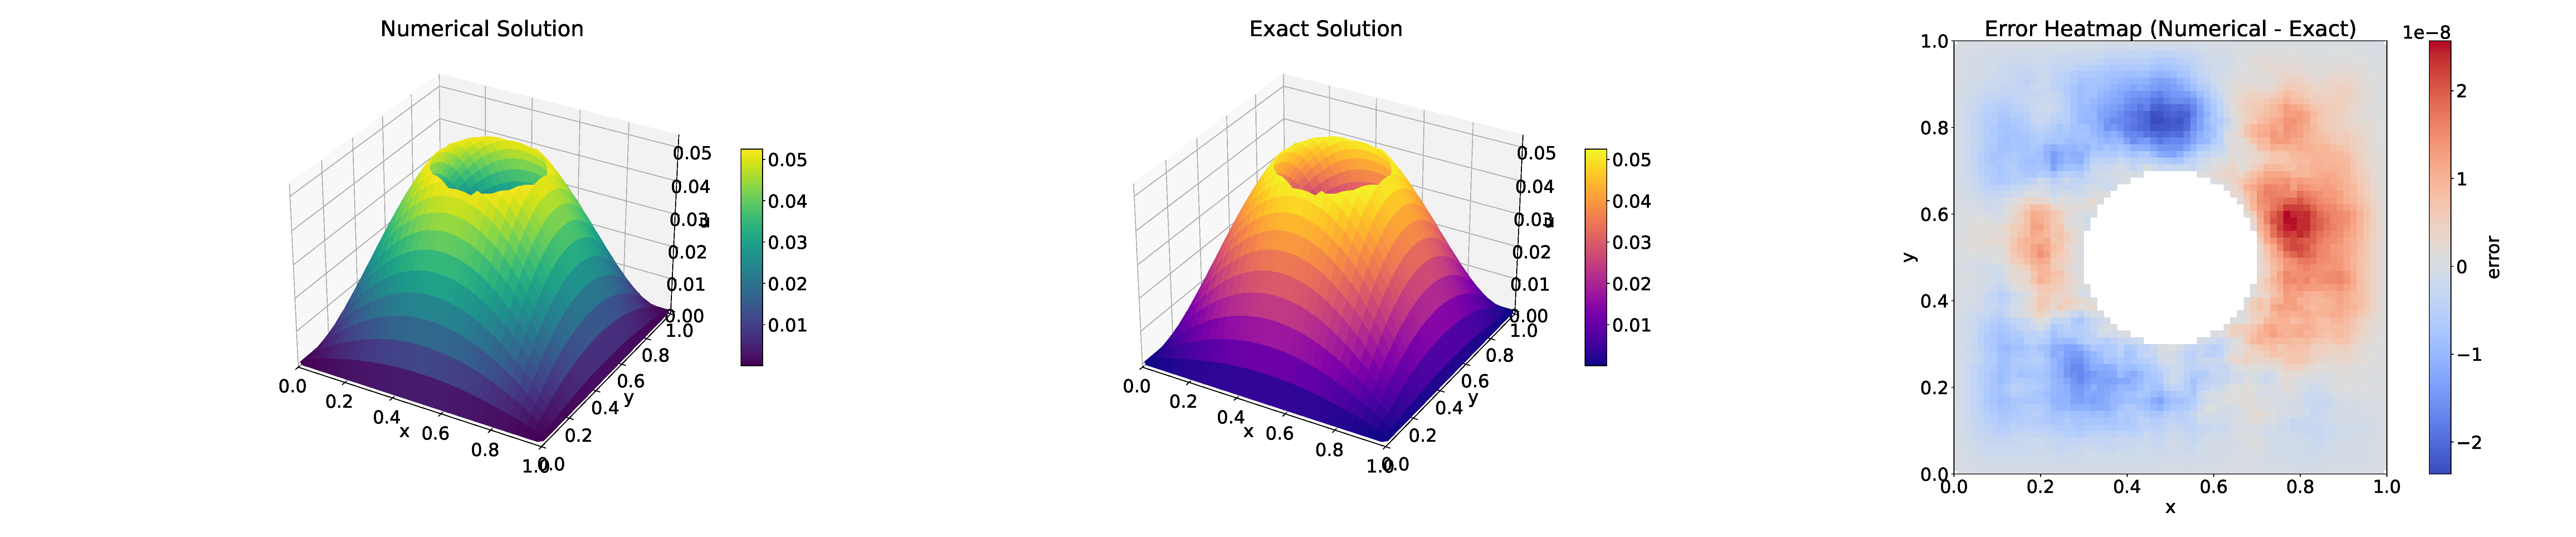
\includegraphics[width=1\textwidth]{figure/PureDirchlet_Circle_Function2.pdf}
    \caption{第二个测试函数：第二种边界假设}
    \label{fig:PureDirchlet_Circle_Function2}
\end{figure}
\par 对于第三种边界假设：矩形左右两边为 Neumann条件，
其余为 Dirichlet 条件、计算域为一个矩形挖去一个圆形
$(x-0.5)^2+(y-0.5)^2=0.04$
\begin{table}[H]
    \centering
    \begin{tabular}{|c|c|c|c|}    
    \hline
    n& 1-norm & 2-norm & $\infty$-norm  \\ \hline
    8&  7.42714e-08&  1.1529e-07 & 3.71573e-07  \\ \hline
    16& 4.57438e-08 & 6.27591e-08 & 1.99328e-07 \\ \hline
    32& 1.09443e-08 & 1.68259e-08 & 6.65748e-08 \\ \hline
    64& 5.89295e-09 & 7.93802e-09 &  2.57769e-08 \\ \hline
    \end{tabular}
\end{table}
\begin{figure}[H]
    \centering
    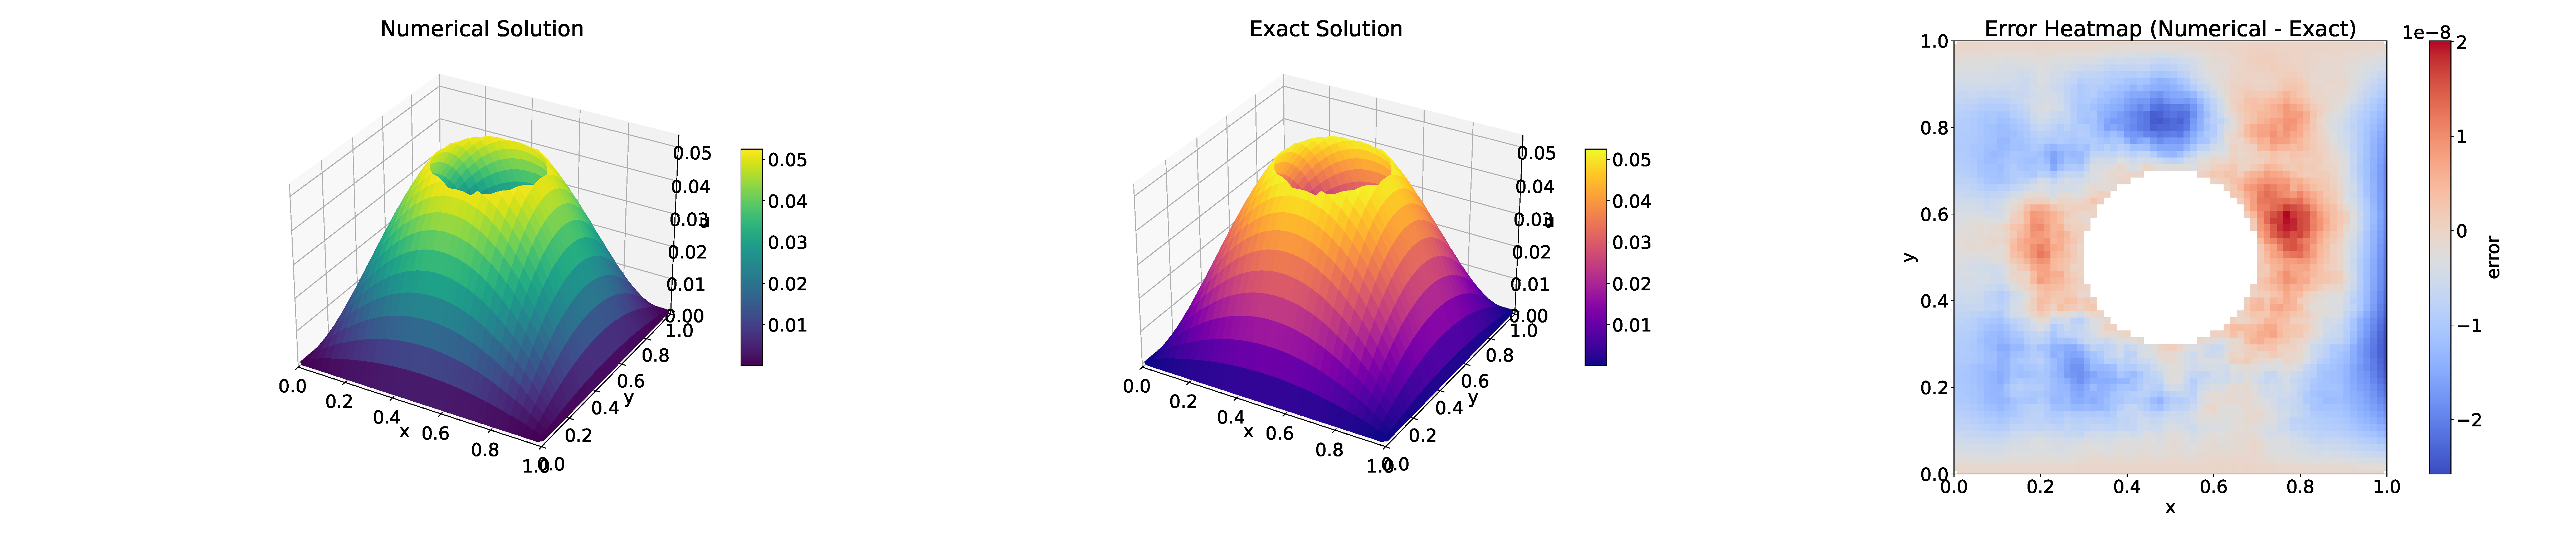
\includegraphics[width=1\textwidth]{figure/MixedNeumann_Rectangle_Function2.pdf}
    \caption{第二个测试函数：第三种边界假设}
    \label{fig:MixedNeumann_Rectangle_Function2}
\end{figure}
\par 对于第四种边界假设：圆形为 Neumann条件，
其余为 Dirichlet 条件、计算域为一个矩形挖去一个圆形
$(x-0.5)^2+(y-0.5)^2=0.04$
\begin{table}[H]
    \centering
    \begin{tabular}{|c|c|c|c|}    
    \hline
    n& 1-norm & 2-norm & $\infty$-norm  \\ \hline
    8&  0.00104445&  0.0014955 & 0.00348838  \\ \hline
    16& 3.96911e-05 & 6.86079e-05 & 0.000326377 \\ \hline
    32& 0.000277468 & 0.00038619 & 0.00100728 \\ \hline
    64& 0.000133844 & 0.000186369 &  0.000499572 \\ \hline
    \end{tabular}
\end{table}
\begin{figure}[H]
    \centering
    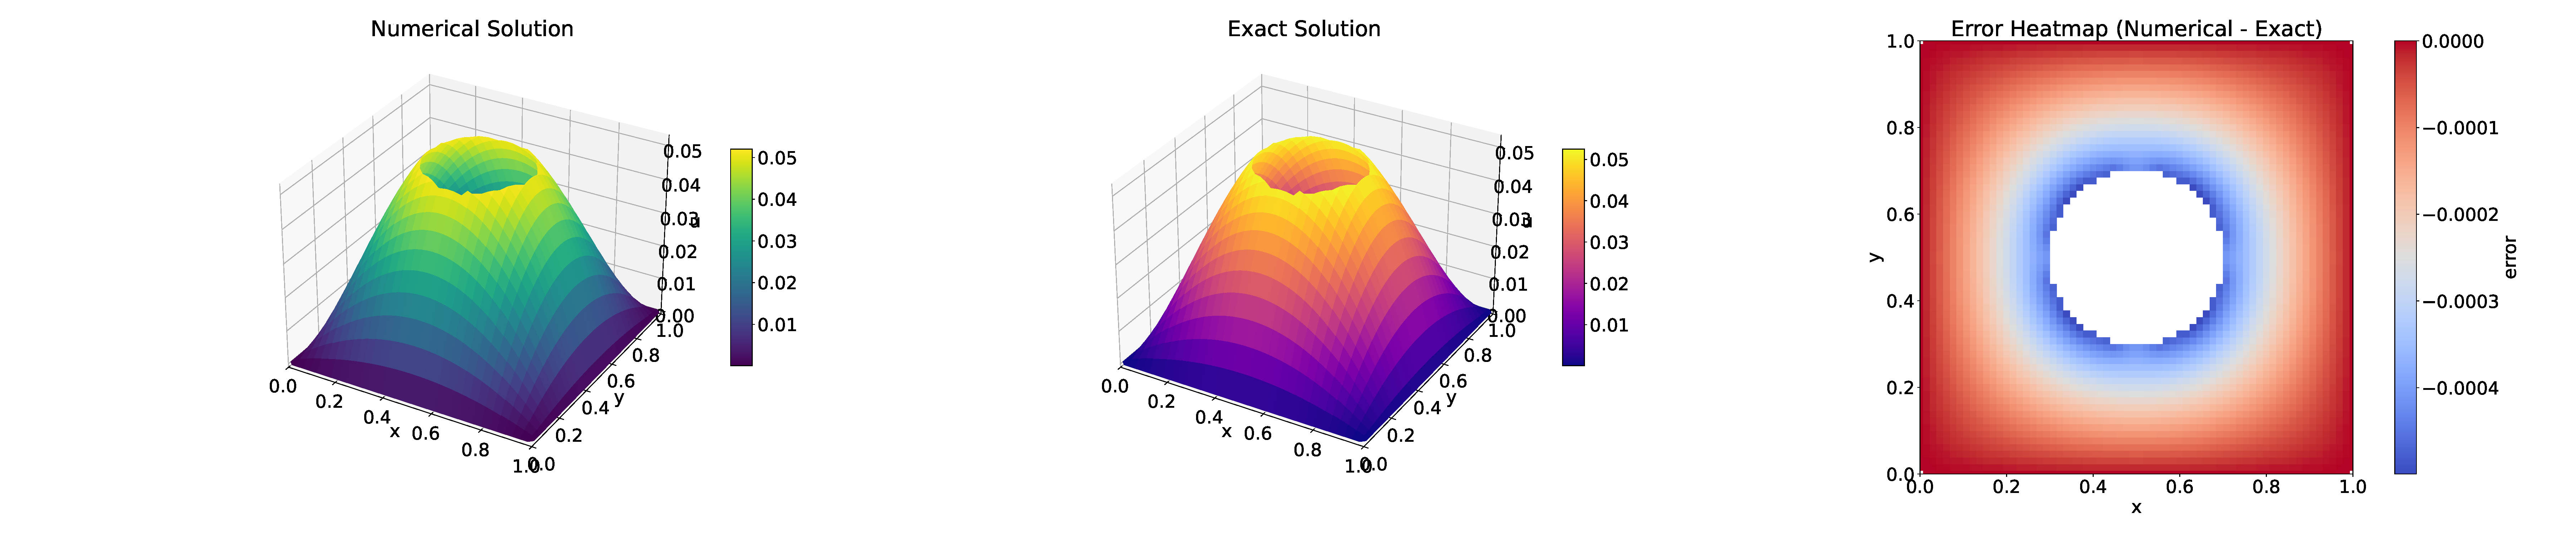
\includegraphics[width=1\textwidth]{figure/MixedNeumann_Circle_Function2.pdf}
    \caption{第二个测试函数：第四种边界假设}
    \label{fig:MixedNeumann_Circle_Function2}
\end{figure}

\subsection{第三个测试函数}

\par 第三个测试函数为：
\begin{equation}
    u(x,y)=\sin x+\sin y
\end{equation}
\par 对于第一种边界假设：纯 Dirichlet 条件、计算域为一个完整的矩形。
\begin{table}[H]
    \centering
    \begin{tabular}{|c|c|c|c|}    
    \hline
    n& 1-norm & 2-norm & $\infty$-norm  \\ \hline
    8&  3.04369e-05&  3.69605e-05 & 6.6088e-05  \\ \hline
    16& 8.45206e-06 & 1.01662e-05 & 1.95948e-05 \\ \hline
    32& 3.41342e-06 & 4.19796e-06 & 8.25092e-06 \\ \hline
    64& 8.56374e-07 & 1.00089e-06 &  1.67482e-06 \\ \hline
    \end{tabular}
\end{table}
\begin{figure}[H]
    \centering
    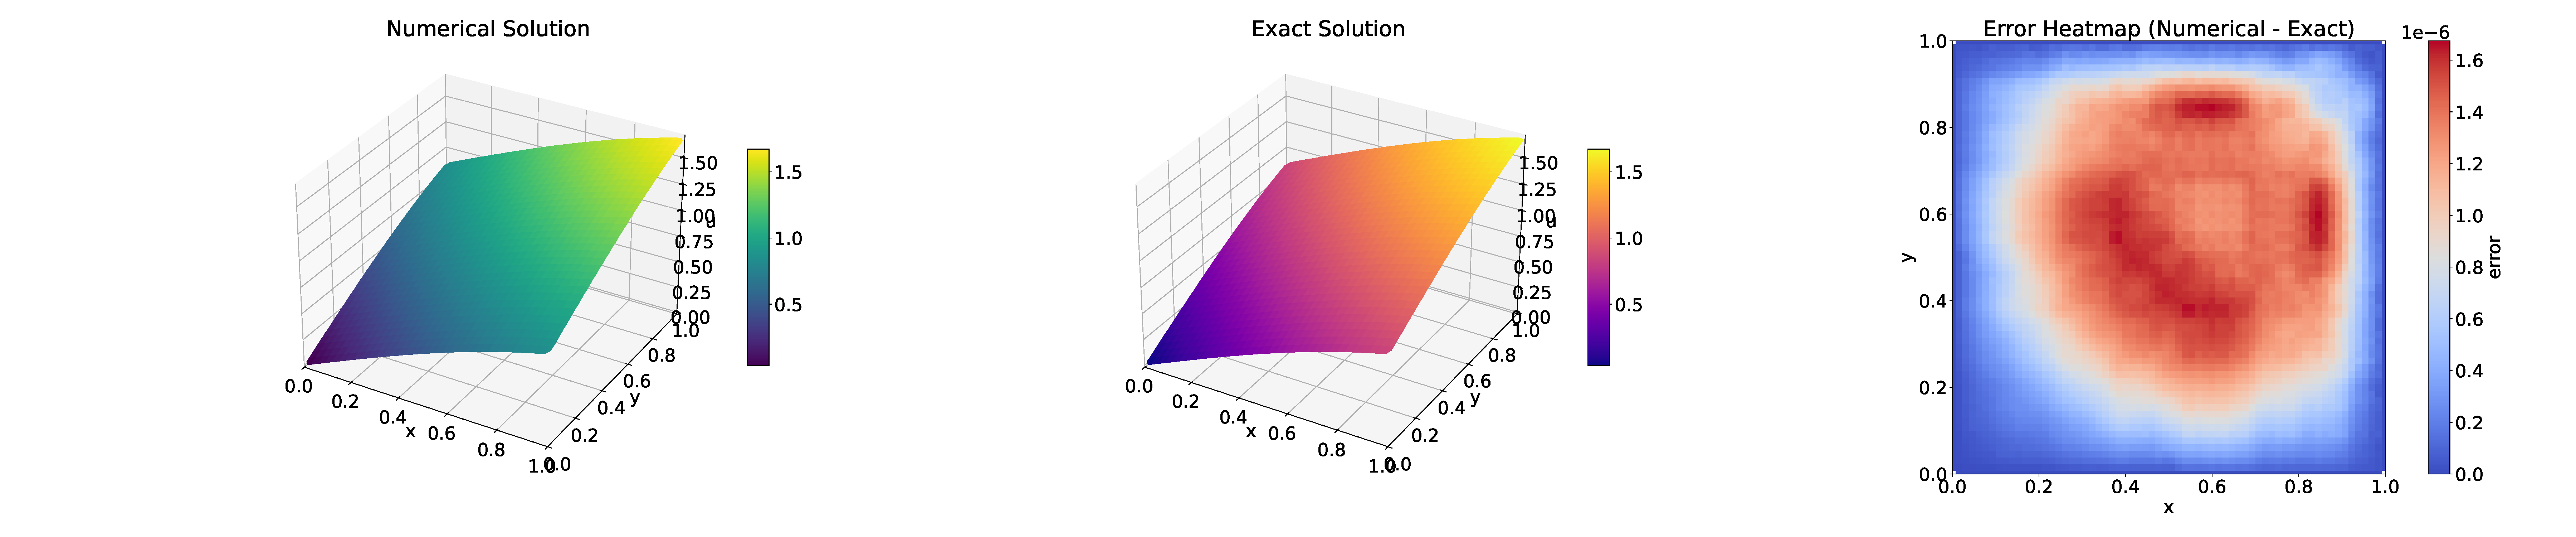
\includegraphics[width=1\textwidth]{figure/PureDirchlet_Rectangle_Function3.pdf}
    \caption{第三个测试函数：第一种边界假设}
    \label{fig:PureDirchlet_Rectangle_Function3}
\end{figure}
\par 对于第二种边界假设：纯 Dirichlet 条件、计算域为一个矩形挖去一个圆形
$(x-0.5)^2+(y-0.5)^2=0.04$
\begin{table}[H]
    \centering
    \begin{tabular}{|c|c|c|c|}    
    \hline
    n& 1-norm & 2-norm & $\infty$-norm  \\ \hline
    8&  1.28536e-05&  2.02474e-05 & 7.02944e-05  \\ \hline
    16& 2.63002e-06 & 3.27149e-06 & 8.59073e-06 \\ \hline
    32& 6.28308e-07 & 8.34922e-07 & 1.93157e-06 \\ \hline
    64& 2.7322e-07 & 3.64443e-07 &  1.07233e-06 \\ \hline
    \end{tabular}
\end{table}
\begin{figure}[H]
    \centering
    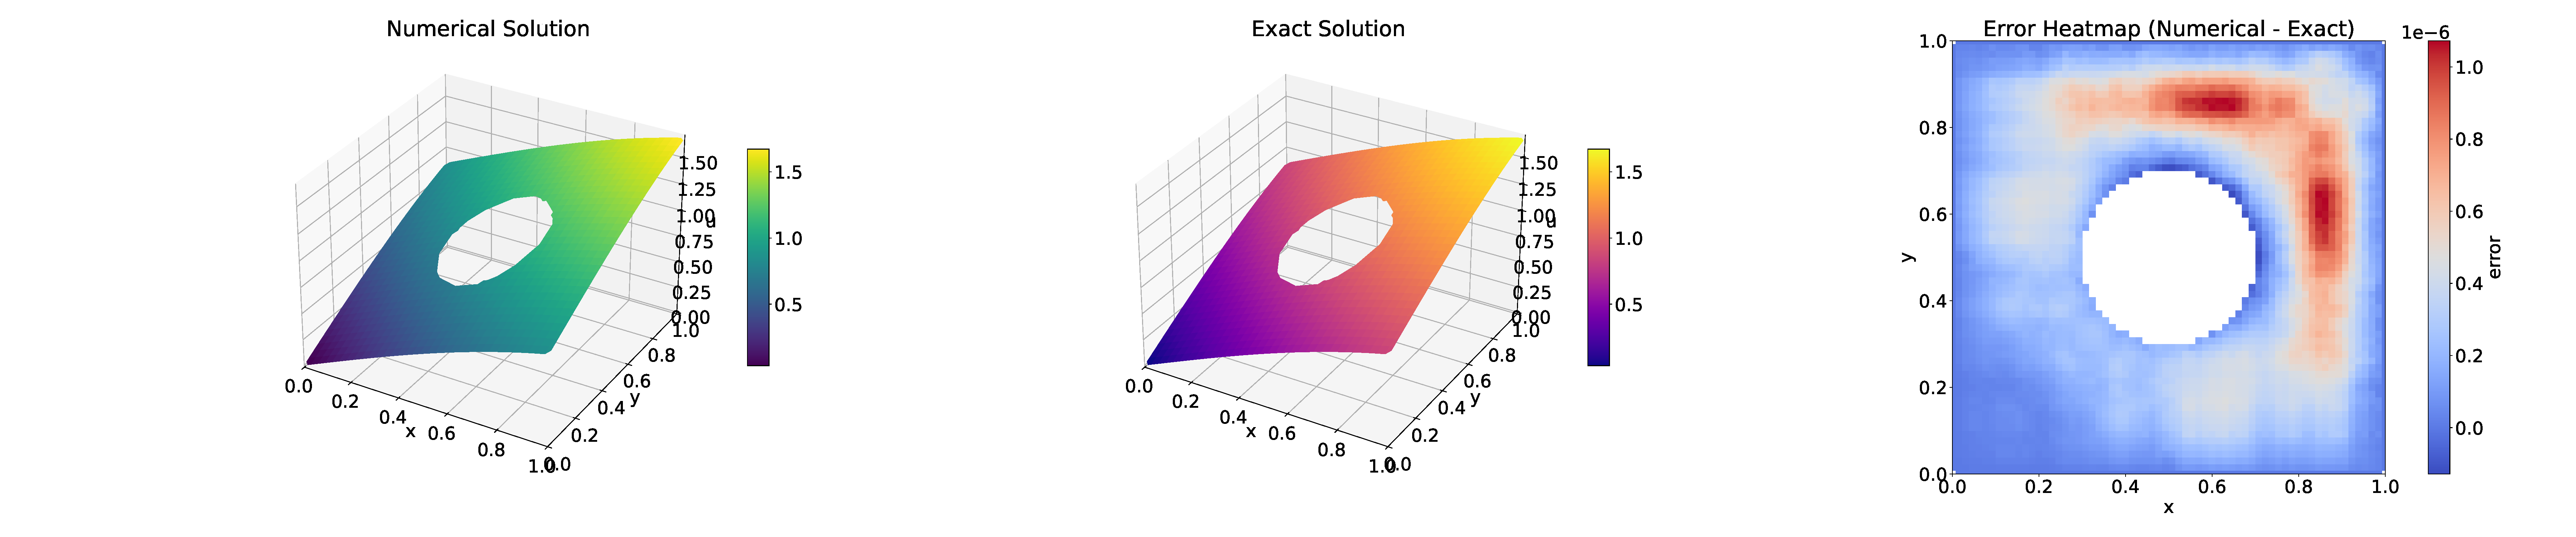
\includegraphics[width=1\textwidth]{figure/PureDirchlet_Circle_Function3.pdf}
    \caption{第三个测试函数：第二种边界假设}
    \label{fig:PureDirchlet_Circle_Function3}
\end{figure}
\par 对于第三种边界假设：矩形左右两边为 Neumann条件，
其余为 Dirichlet 条件、计算域为一个矩形挖去一个圆形
$(x-0.5)^2+(y-0.5)^2=0.04$
\begin{table}[H]
    \centering
    \begin{tabular}{|c|c|c|c|}    
    \hline
    n& 1-norm & 2-norm & $\infty$-norm  \\ \hline
    8&  0.000138875&  0.000198328 & 0.000510292  \\ \hline
    16& 3.71881e-05 & 5.37962e-05 & 0.000152206 \\ \hline
    32& 8.81228e-06 & 1.29914e-05 & 3.9723e-05 \\ \hline
    64&  2.4149e-06 & 3.47884e-06 &  1.02202e-05 \\ \hline
    \end{tabular}
\end{table}
\begin{figure}[H]
    \centering
    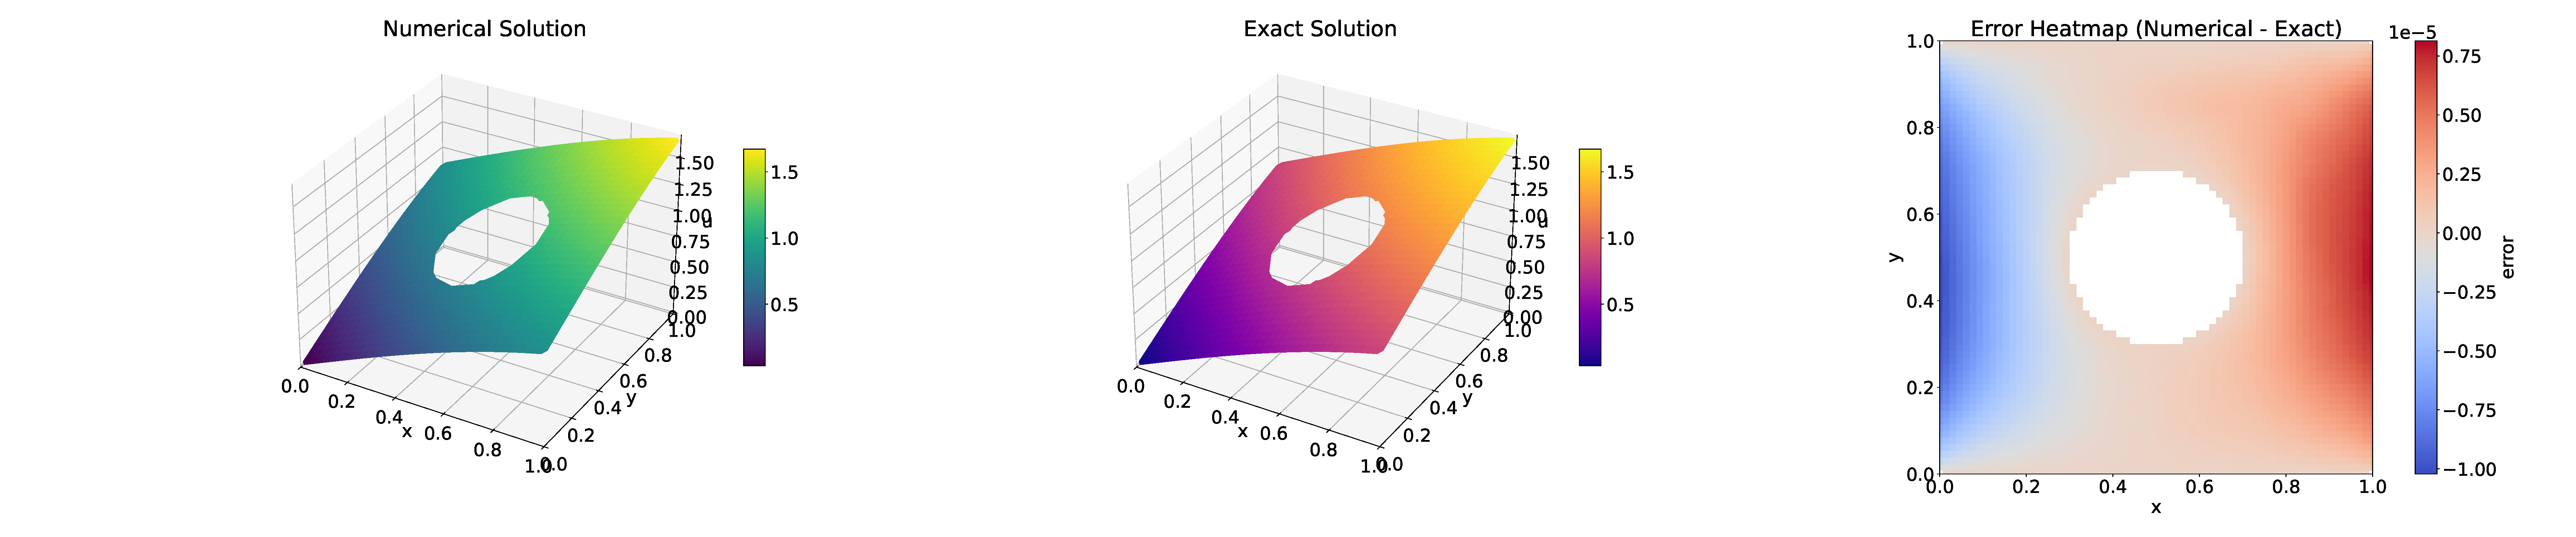
\includegraphics[width=1\textwidth]{figure/MixedNeumann_Rectangle_Function3.pdf}
    \caption{第三个测试函数：第三种边界假设}
    \label{fig:MixedNeumann_Rectangle_Function3}
\end{figure}
\par 对于第四种边界假设：圆形为 Neumann条件，
其余为 Dirichlet 条件、计算域为一个矩形挖去一个圆形
$(x-0.5)^2+(y-0.5)^2=0.04$
\begin{table}[H]
    \centering
    \begin{tabular}{|c|c|c|c|}    
    \hline
    n& 1-norm & 2-norm & $\infty$-norm  \\ \hline
    8&  0.00116519&  0.00170533 & 0.00502059  \\ \hline
    16& 7.46603e-05 & 0.000116561 & 0.00053906 \\ \hline
    32& 0.000312729 & 0.000442147 &  0.00146427 \\ \hline
    64& 0.00014951 & 0.000210968 &  0.000708359 \\ \hline
    \end{tabular}
\end{table}
\begin{figure}[H]
    \centering
    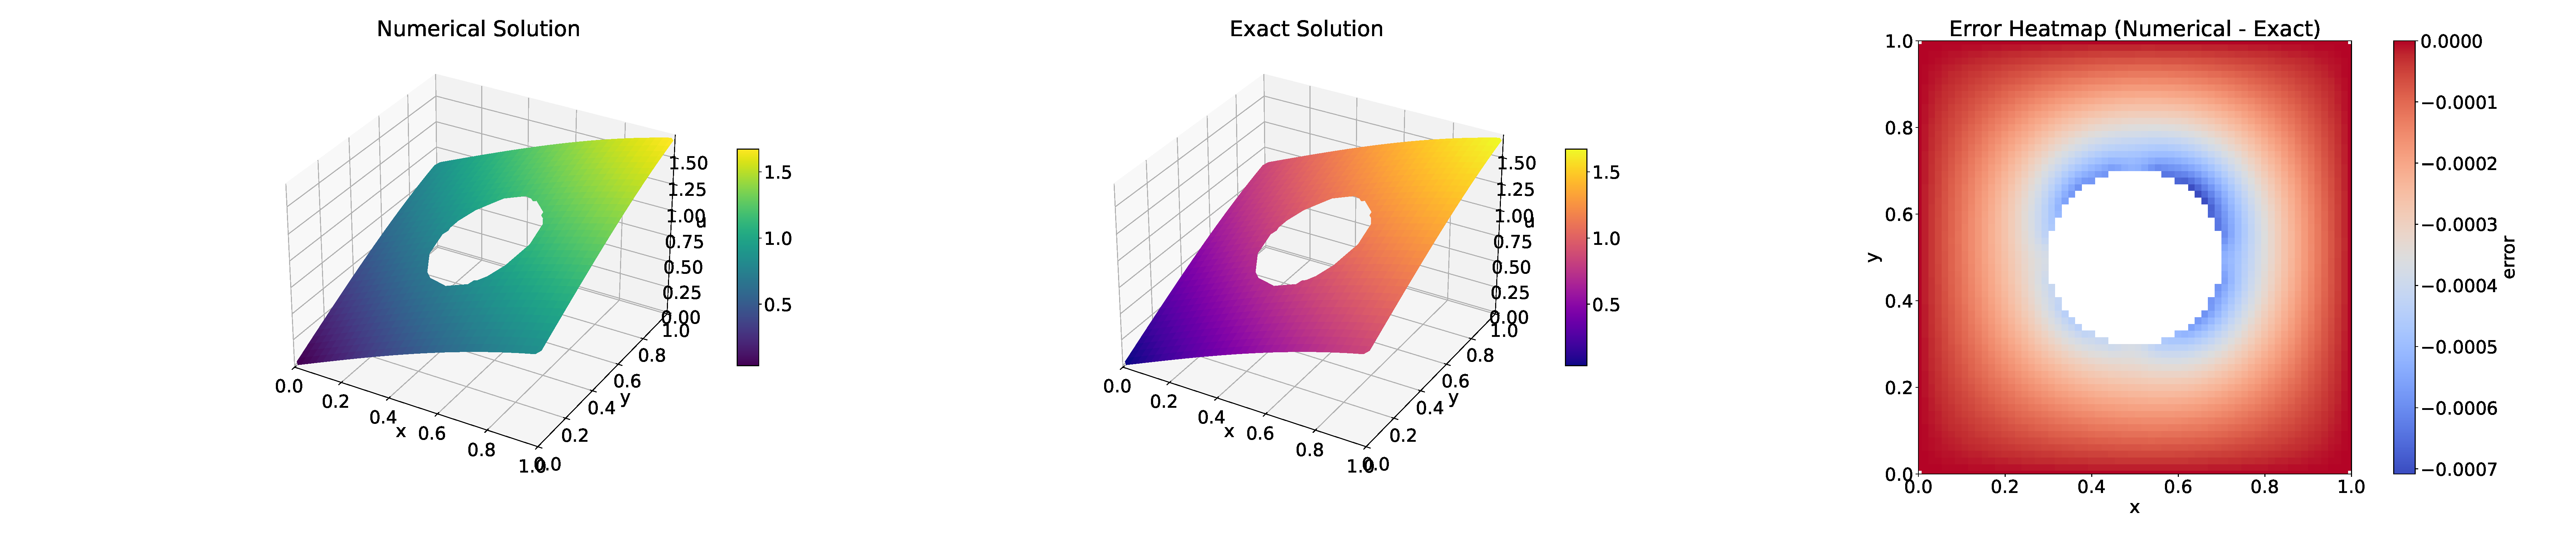
\includegraphics[width=1\textwidth]{figure/MixedNeumann_Circle_Function3.pdf}
    \caption{第三个测试函数：第四种边界假设}
    \label{fig:MixedNeumann_Circle_Function3}
\end{figure}

\subsection{结果分析}

\par 从第一个和第三个测试函数的数值结果可以看出，
对于矩形规则边界的 Dirichlet 条件和 Neumann 条件，无穷范数呈2阶收敛；
而对于圆形不规则边界的 Dirichlet 条件，无穷范数呈2阶收敛，
对于圆形不规则边界的 Neumann 条件，无穷范数则呈1阶收敛。
第二个测试函数由于是多项式函数，因此在
除了第四种边界假设以外的其他三种边界假设下都只有机器精度误差。

\subsection{更多测试边界}

\par 均采用第一个测试函数，并选取 Dirichlet 条件
只为了测试不同位置的圆形下程序的正确性。
\begin{figure}[H]
    \centering
    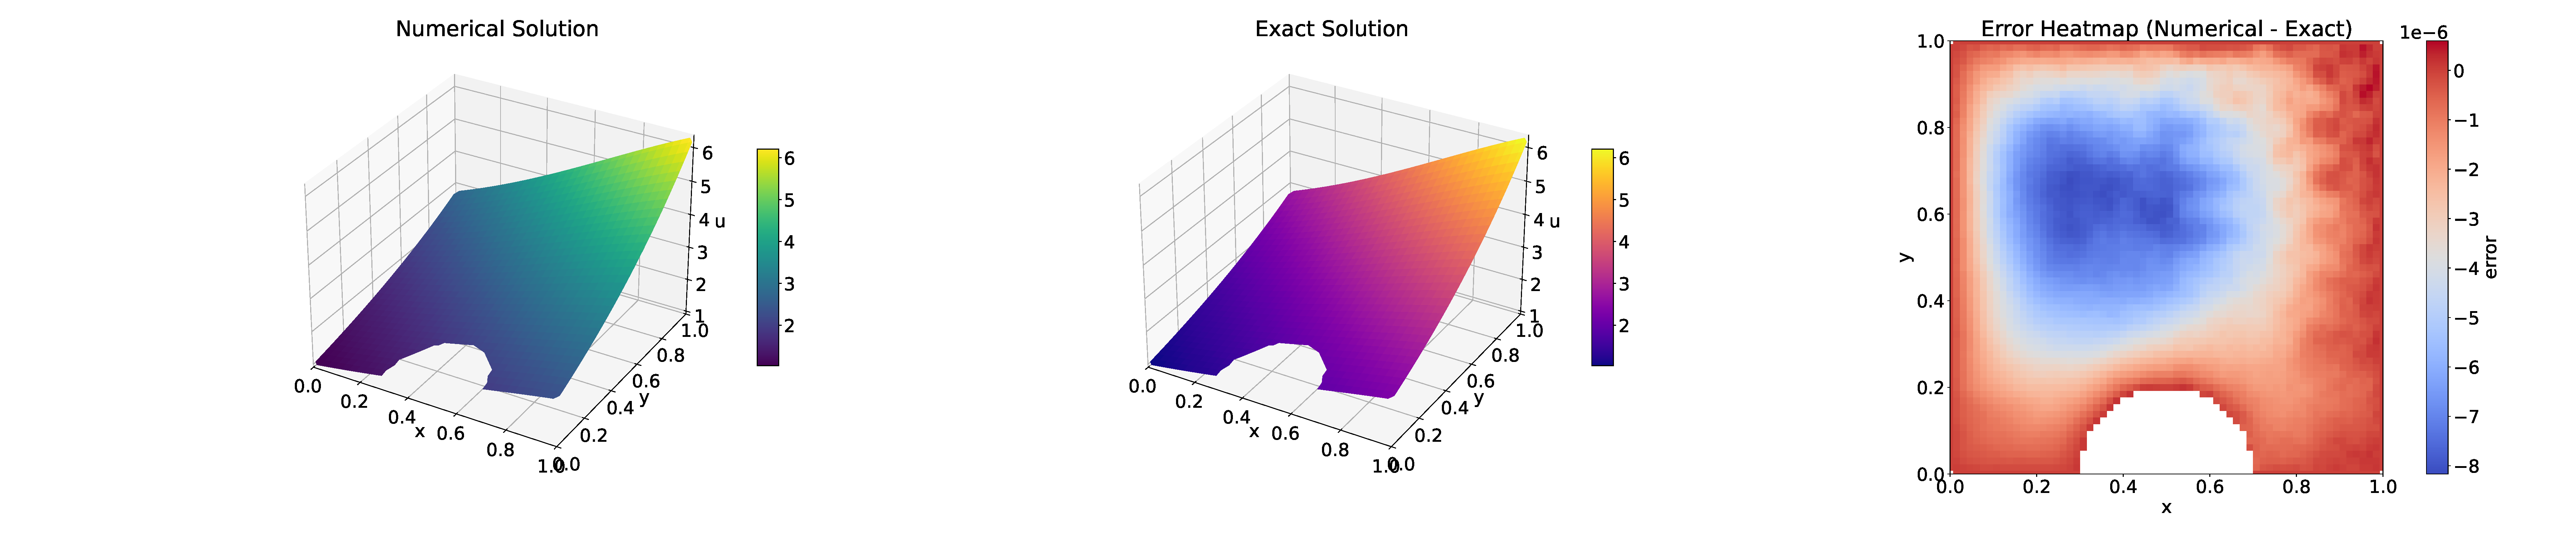
\includegraphics[width=1\textwidth]{figure/MoreExample_1.pdf}
    \caption{$(x-0.5)^2+y^2=0.04$}
    \label{fig:MoreExample_1}
\end{figure}
\begin{figure}[H]
    \centering
    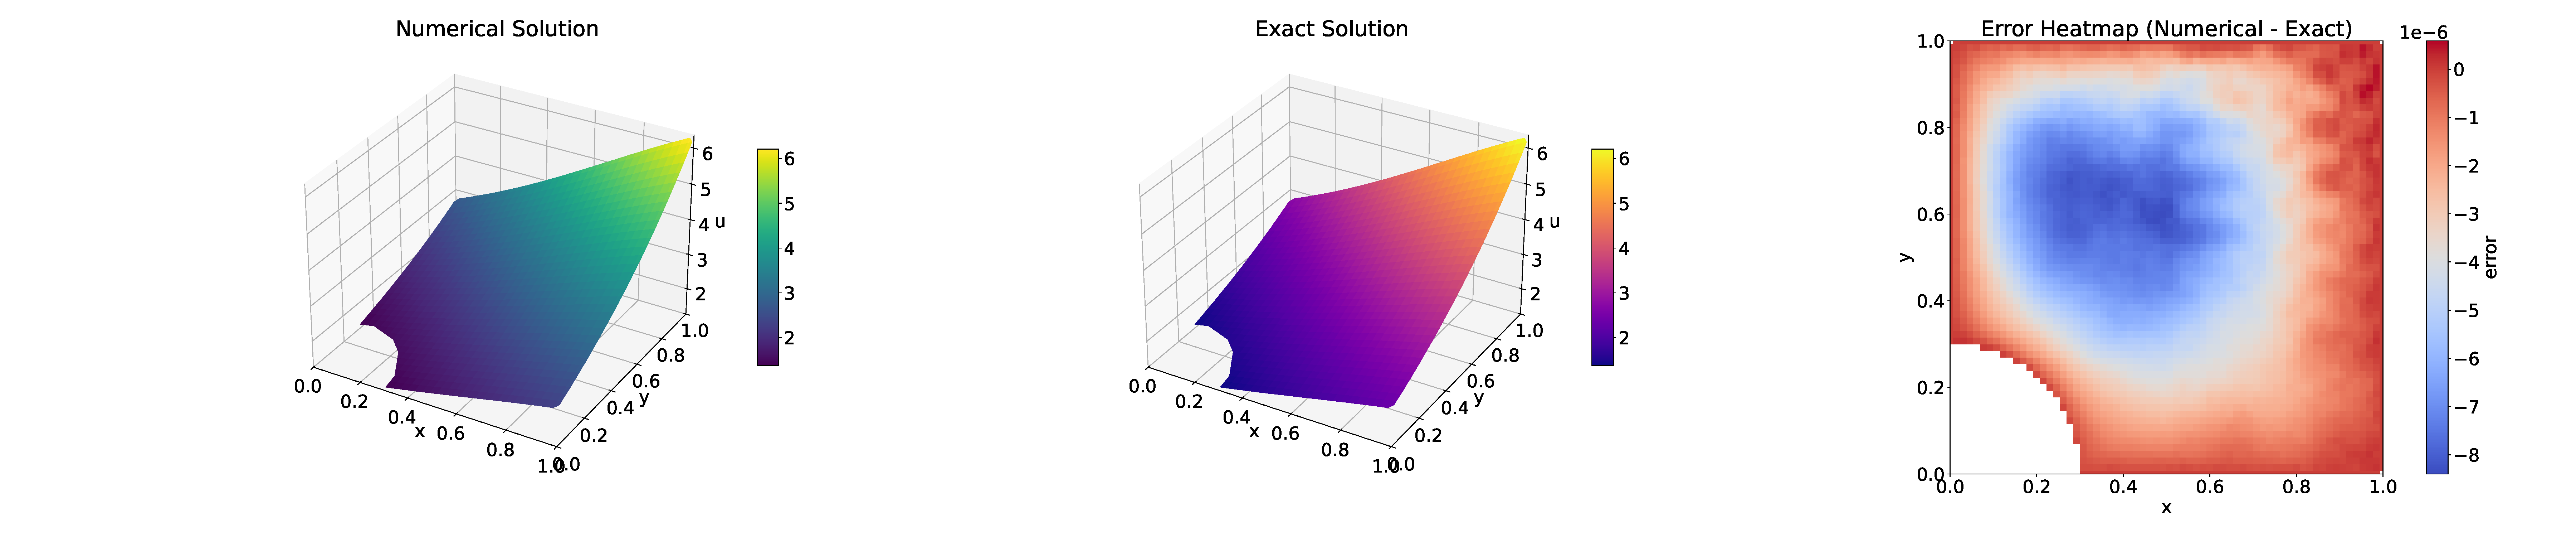
\includegraphics[width=1\textwidth]{figure/MoreExample_2.pdf}
    \caption{$x^2+y^2=0.09$}
    \label{fig:MoreExample_2}
\end{figure}
\begin{figure}[H]
    \centering
    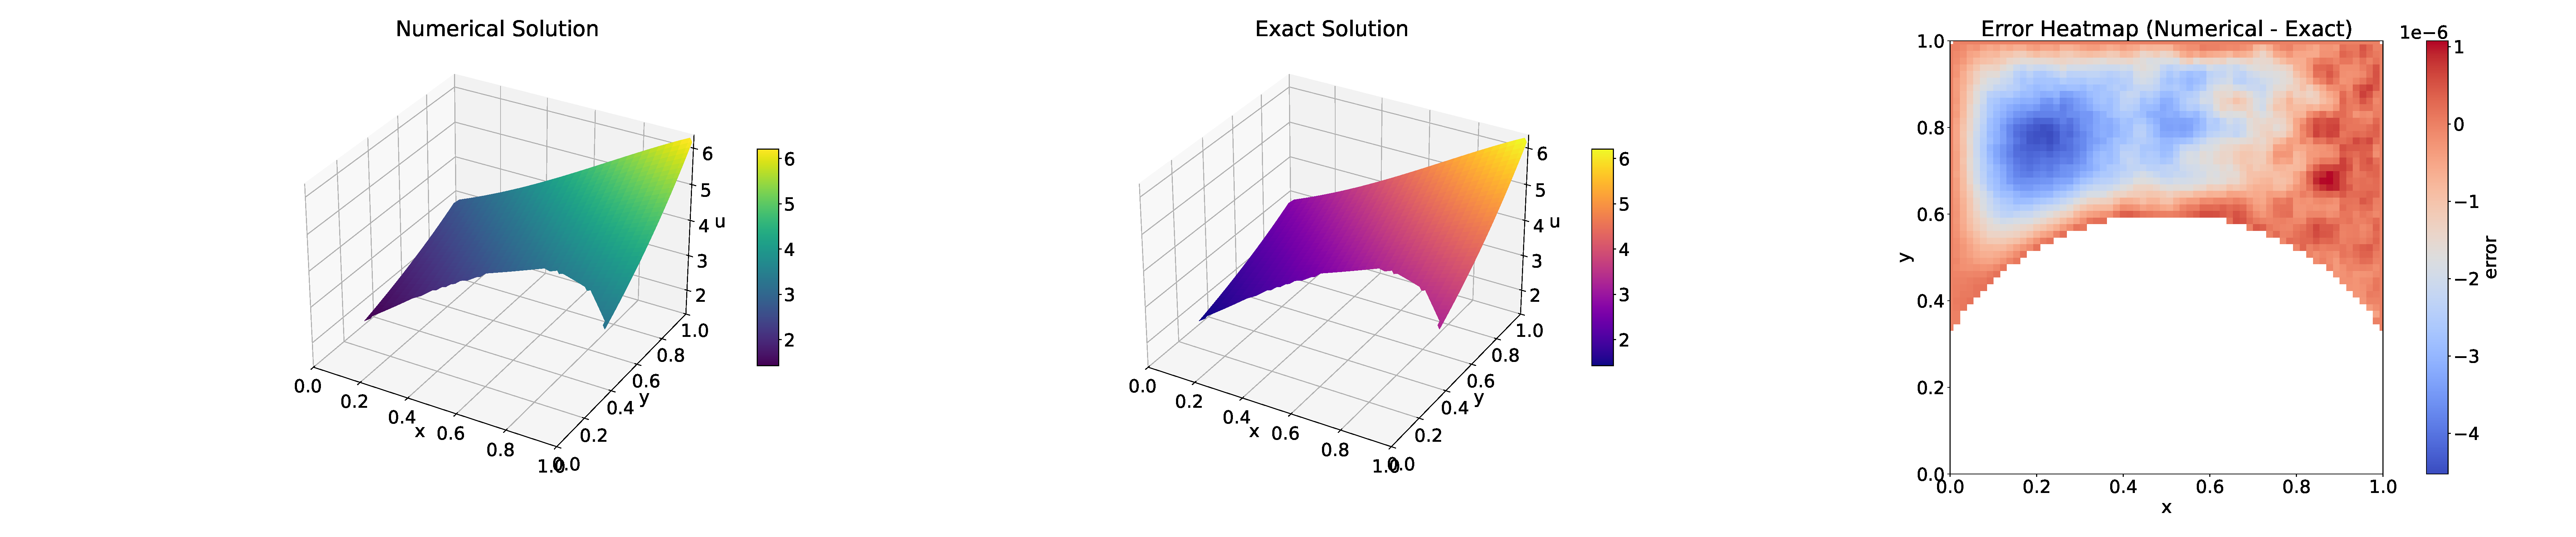
\includegraphics[width=1\textwidth]{figure/MoreExample_3.pdf}
    \caption{$(x-0.5)^2+y^2=0.36$}
    \label{fig:MoreExample_3}
\end{figure}
\begin{figure}[H]
    \centering
    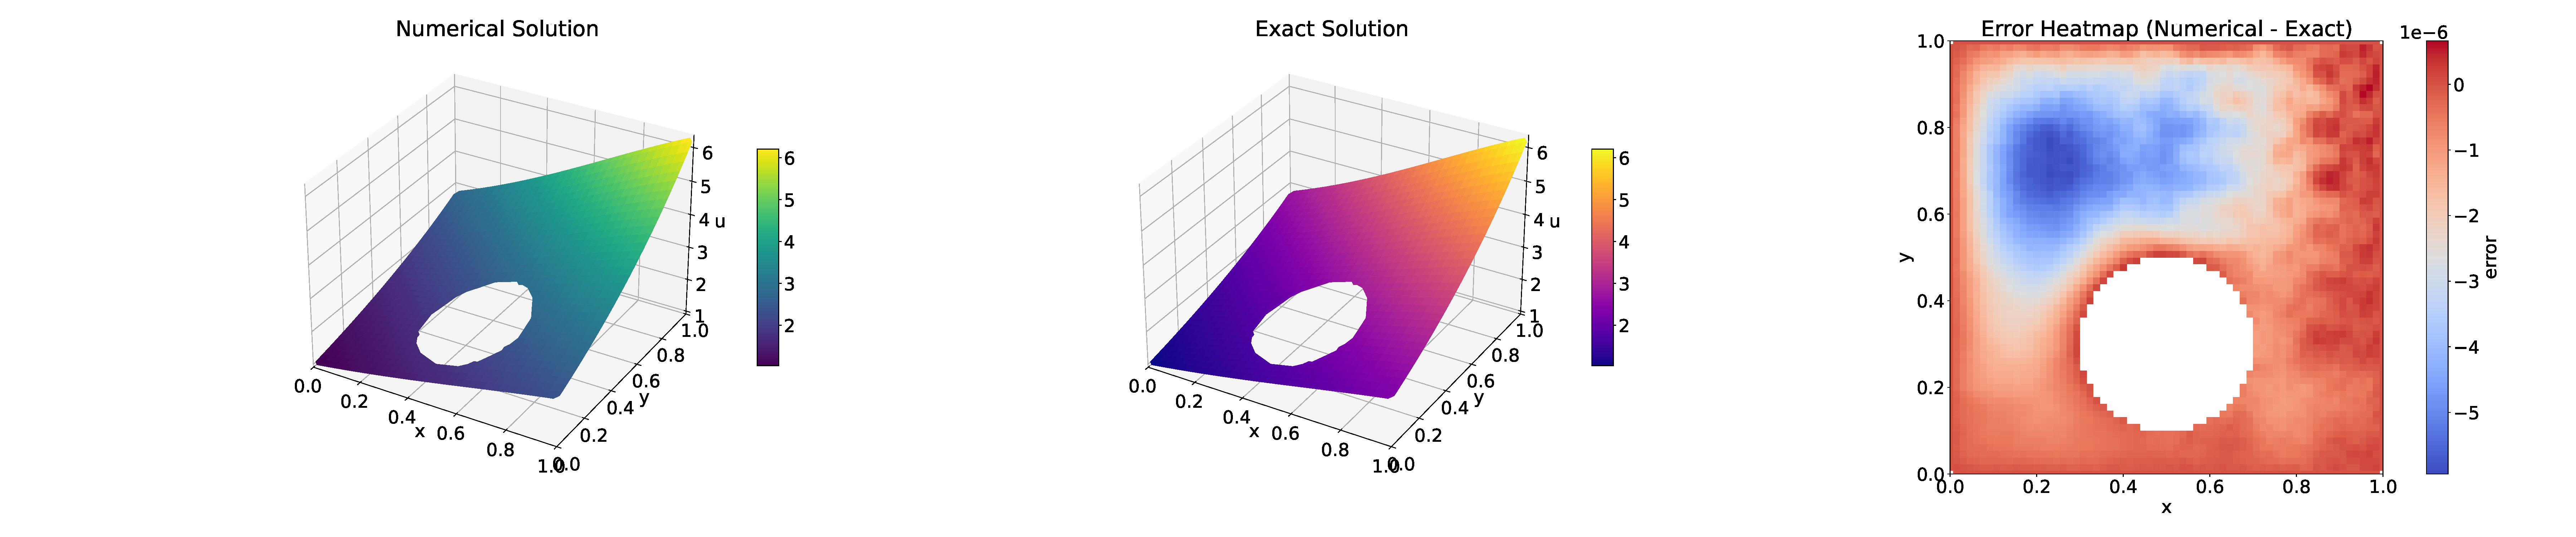
\includegraphics[width=1\textwidth]{figure/MoreExample_4.pdf}
    \caption{$(x-0.5)^2+(y-0.3)^2=0.04$}
    \label{fig:MoreExample_4}
\end{figure}

% ===============================================

\printbibliography

\end{document}